% \PassOptionsToPackage{table}{xcolor}
\documentclass[11pt]{beamer}
\usepackage[utf8]{inputenc}
\usepackage[english]{babel}
\usepackage{amsmath}
\usepackage{amsfonts}
\usepackage{amssymb}
\usepackage{graphicx}
\usepackage{tikz}
\usepackage{algorithm}
\usepackage{algorithmic}
\usepackage{silence,lmodern}
\usepackage{csquotes}
\usepackage[backend=bibtex, bibencoding=ascii, style=authoryear, doi=false, isbn=false,url=false, uniquename=init, giveninits=true]{biblatex}
\usepackage{multimedia}
\usepackage{dirtytalk}
\usepackage{pgfplotstable,booktabs,longtable}
\usepackage{grffile}
\usepackage{marvosym} % color image
\WarningFilter{biblatex}{Patching footnotes failed}


% \mode<presentation>
% {
    \usetheme[hideothersubsections]{PaloAlto}
    % \usecolortheme{beaver}
% }
\usetikzlibrary{calc,trees,positioning,arrows,chains,shapes.geometric,
decorations.pathreplacing,decorations.pathmorphing,
shapes,matrix,shapes.symbols,plotmarks,decorations.markings,
shadows,shapes.geometric,arrows}

\setbeamercolor{logo}{bg=white}  %controls the color of the logo area
\setbeamerfont{footnote}{size=\tiny}

% \addbibresource{library.bib}

\makeatletter
\setlength{\beamer@headheight}{.9cm}
\makeatother

\author{S M Al Mahi}
\title[ECEN-5283 Computer Vision]{Project 4: \\Image Segmentation Using\\K-means and EM}
\setbeamercovered{transparent} 
\setbeamertemplate{navigation symbols}{}


\logo{
\includegraphics[width=1cm]{Oklahoma_State_University_logo.png}}
\institute{Oklahoma State University} 
\date{\today} 
\subject{}
\begin{document}

\setbeamertemplate{sidebar left}{}
\begin{frame}
\titlepage
\end{frame}

\newpage
\setbeamertemplate{sidebar left}[sidebar theme]
\section{Project Objective}
\begin{frame}
\frametitle{Project Objective}
	\begin{block}{Objectives}
	\begin{enumerate}
		\item Implement K-means and Expectation Maximization(EM) algorithms
		\item Apply them for image segmentation 
		\item Analyze the result with different initialization
		\item Apply them on Gray and Colored image
	\end{enumerate}
	\end{block}
\end{frame}

\section{Technical Background}
\subsection{K-means}
\begin{frame}
\frametitle{K-means}
{\bf K-means clustering algorithm}

\begin{enumerate}

\setcounter{enumi}{-1}

\item Start with initial guesses for cluster centers (centroids)
\item For each data point, find closest cluster center (partitioning step)
\item Replace each centroid by average of data points in its partition
\item Iterate 1+2 until convergence

\end{enumerate}

\end{frame}
\begin{frame}
Given a set of observations $y$ into a $K$ clusters. 

\[
x_i^{(t)} = argmin_i \big \{ y_i : \big \| y_i - \mu^{(t)}_k \big \|^2  \ \forall_{k,i}, 1 \le j \le K, 1 \le i \le N \big\}
\label{eqn:kmeans_assign_step}
\]

Afterwards, the center-points are repositioned by calculating the mean of the assigned observations to the respective center-points

\[
\mu^{(t+1)}_k = \frac{1}{N_k} \sum_{x_i \in x^{(t)}_k} x_i
\]


\end{frame}

\begin{frame}
\frametitle{K-means}
$y_i = (y_{i1}, ... y_{id})$:

If centroids are $m_1, m_2, ... m_k$, and partitions are

$c_1, c_2, ... c_k$, then one can show that K-means converges to a {\it local} minimum of

\[
\sum^K_{k=1} \sum_{i\in c_k} || x_i - m_k ||^2
\]

\end{frame}

\subsection{EM}
\begin{frame}
\frametitle{EM algorithm for Gaussian mixtures}
\begin{itemize}
\item EM can be thought of a probabilistic version of K-means
\item Instead of hard assigning a data point to a cluster it assigns a probability
\item The mean an covariance for Gaussian often initialized using fast K-means clustering
\item EM is a two step algorithm
\end{itemize}

\end{frame}

\begin{frame}
\frametitle{EM algorithm}
E-Step:\\
\[\begin{split}
\gamma (z_k) = p(z_k=1|y) 
&= \frac{p(y|z_k=1)p(z_k=1)}{p(y)} \\
&= \frac{\alpha_k\mathcal{N}(y|\mu_k, \Sigma_k)}{\Sigma^K_{j=1}\pi_j\mathcal{N}(y|\mu_j,\Sigma_j)}
\end{split}
\]
M-step:\\
\[
\mu_k=\frac{\Sigma^{N}_{n=1}\gamma(z_{nk})y_n}{\Sigma^{N}_{n=1}\gamma(z_{nk})}
\]
\[
\Sigma_k=\frac{1}{N_k}\gamma_k(z_{nk})(y_n-\mu_k)(y_n-\mu_k)^T
\]
\end{frame}

\begin{frame}
The objective function for EM is
\[
lnp(X|\alpha,\mu,\Sigma)=\Sigma^N_{n=1}ln\{\Sigma^K_{k=1}\alpha_k
\mathcal{N}(x_n|\mu_k,\Sigma_k)\}
\]
\end{frame}

\section{Experiment and Results}
% \begin{frame}
% \frametitle{Retinal Image Cock wise 1 to 4}
% \begin{columns}[T] % align columns
% \begin{column}{\textwidth}
% \centering
% 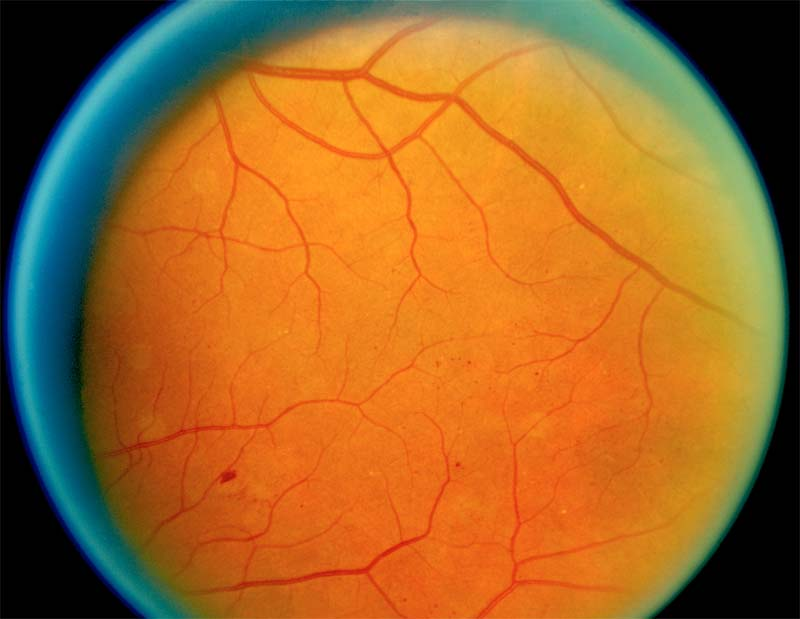
\includegraphics[width=.45\textwidth, height=.45\textheight]{retina1.jpg}\vspace{1pt}
% 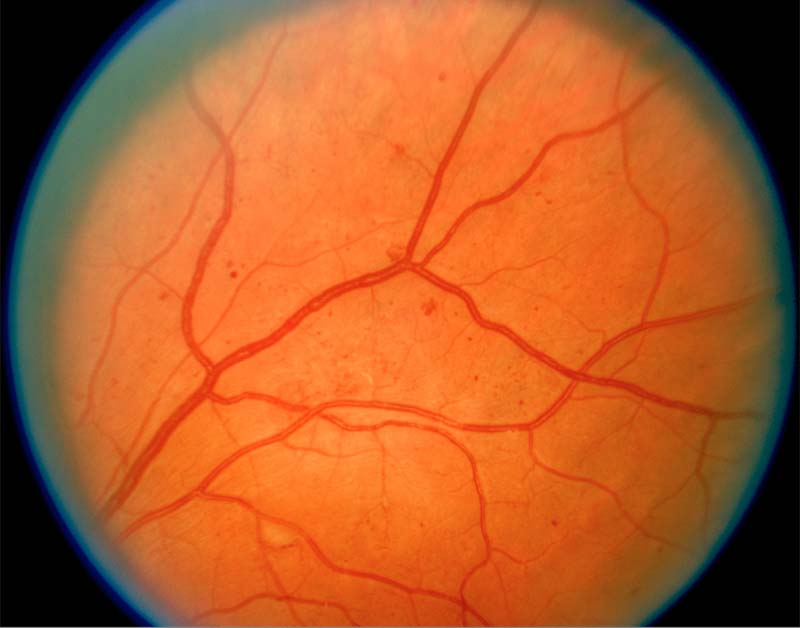
\includegraphics[width=.45\textwidth, height=.45\textheight]{retina2.jpg}\vfill
% 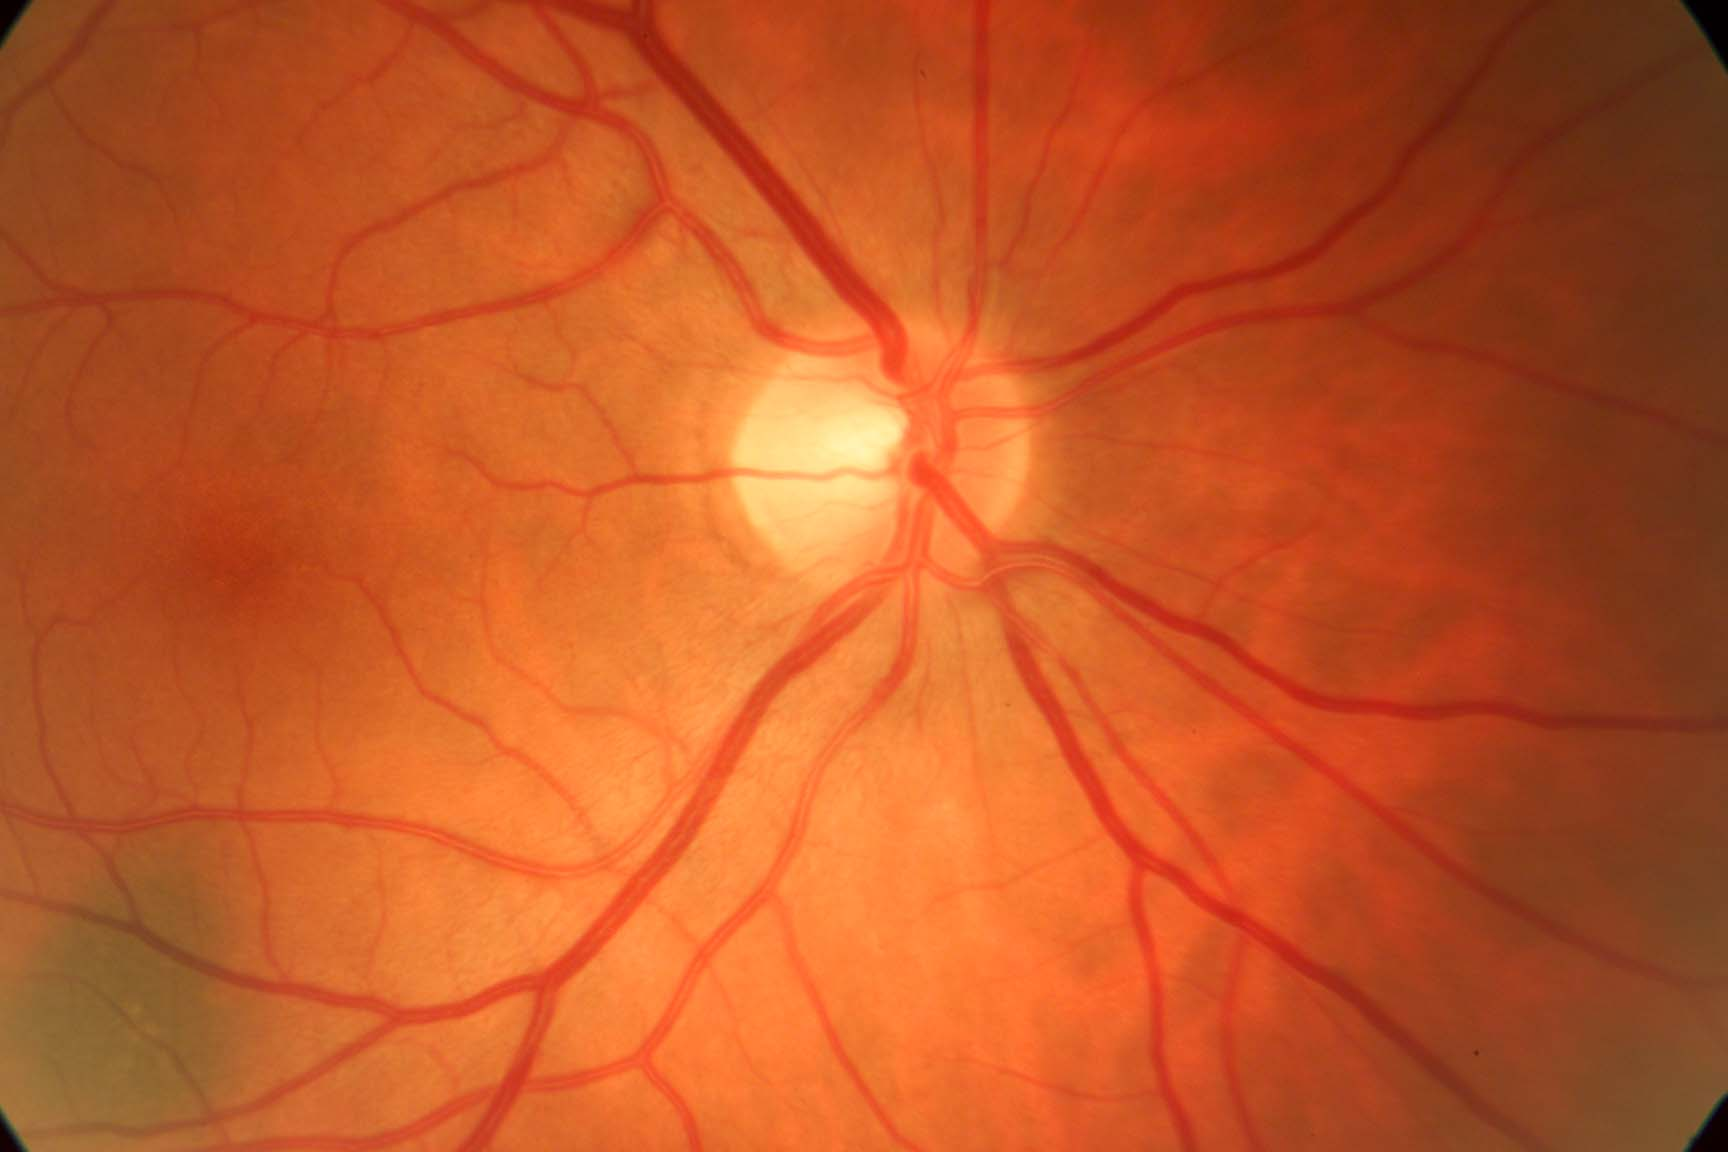
\includegraphics[width=.45\textwidth, height=.45\textheight]{retina3.jpg}\vspace{1pt}
% 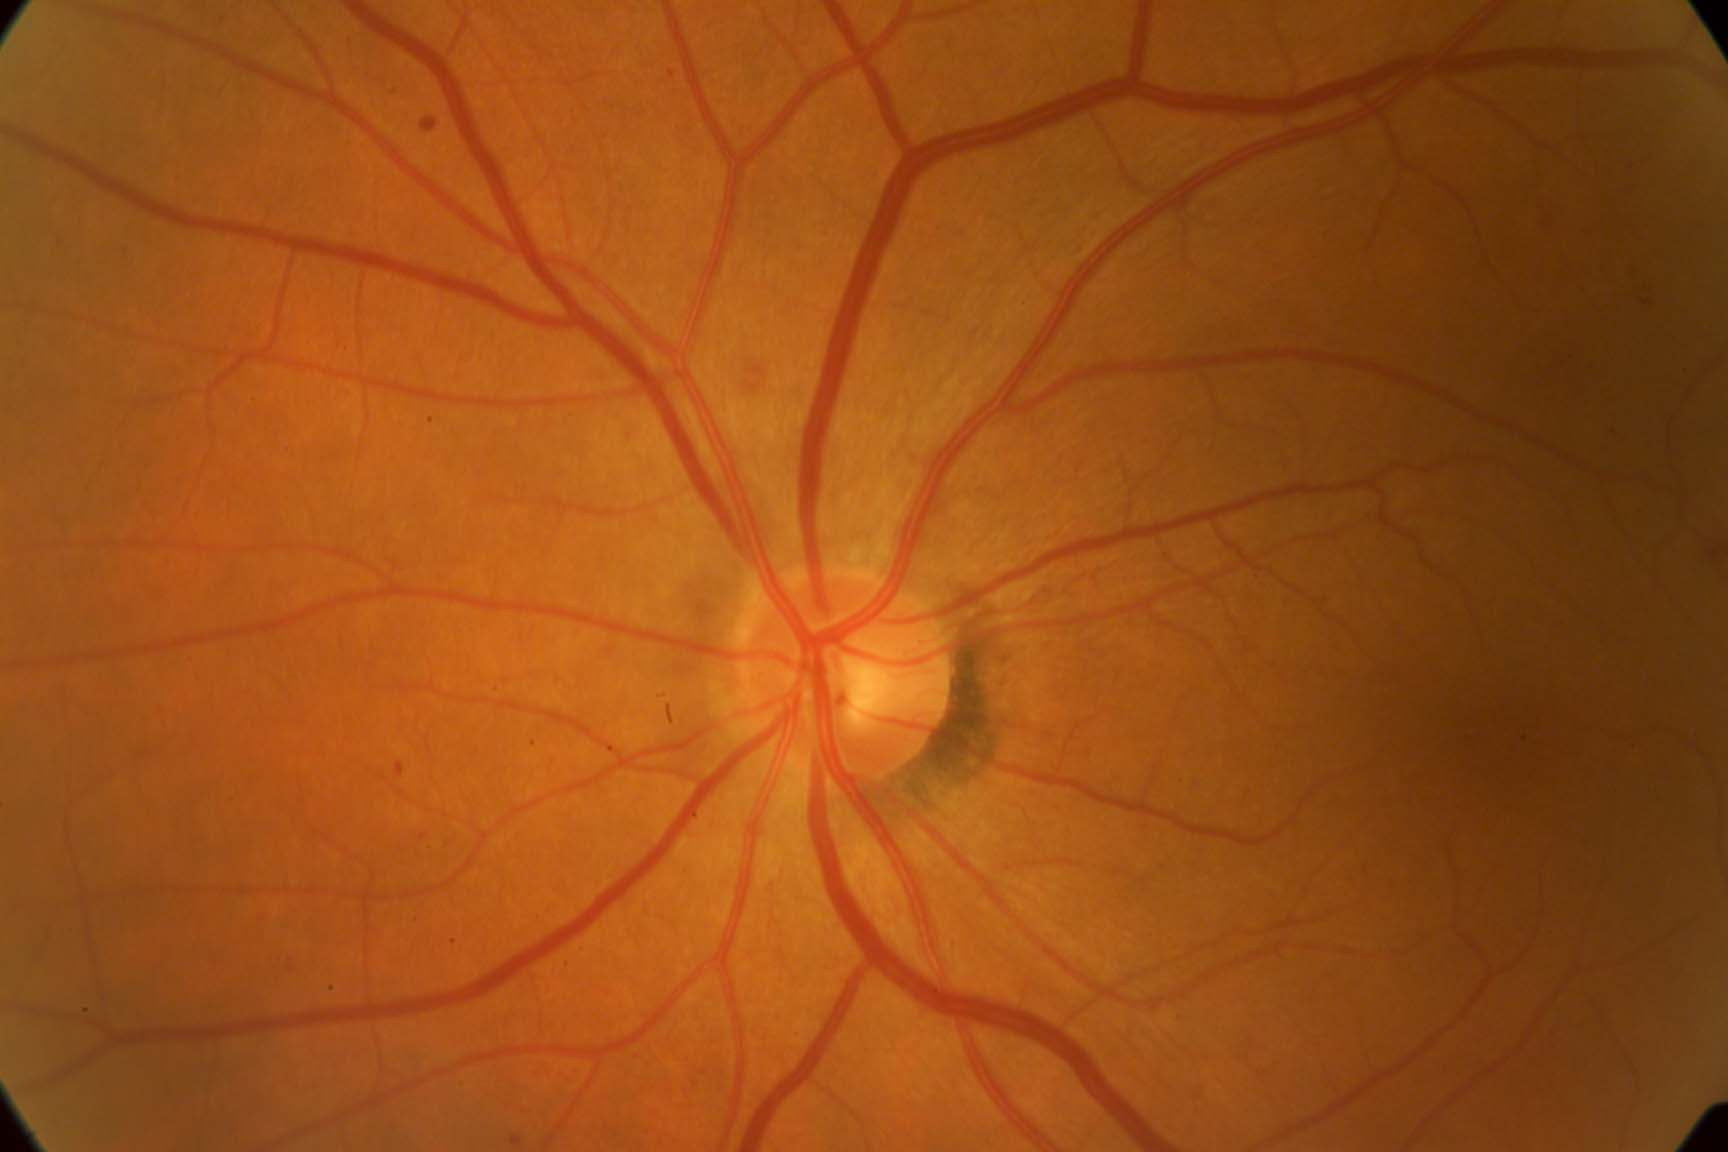
\includegraphics[width=.45\textwidth, height=.45\textheight]{retina4.jpg}\vfill
% \end{column}
% \end{columns}\vfill
% \end{frame}

\subsection{K-means}
\begin{frame}
\frametitle{Test Image Mosaic A}
\begin{columns}[onlytextwidth]
\begin{column}{.45\textwidth}
\begin{figure}
  \colorbox{gray!20}{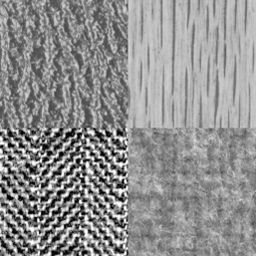
\includegraphics[width=.9\textwidth]{mosaicA.png}}
  \caption{Test Image}
\end{figure}
\end{column}
\hfill
\begin{column}{.45\textwidth}
\begin{figure}
  \colorbox{gray!20}{
\includegraphics[width=.9\textwidth]{mapA.png}}
  \caption{Ground Truth}
\end{figure}
\end{column}
\end{columns}
\end{frame}

\begin{frame}
\frametitle{K-means Initializations for A}
\begin{columns}[onlytextwidth]
\begin{column}{.45\textwidth}
\begin{figure}
  \includegraphics[width=.9\textwidth]{figs/kmeansA/kmeansgood_0_prog_A.png}
  \caption{Good}
\end{figure}
\end{column}
\hfill
\begin{column}{.45\textwidth}
\begin{figure}
  \includegraphics[width=.9\textwidth]{figs/kmeansA/kmeansbad_0_prog_A.png}
  \caption{Bad}
\end{figure}
\end{column}
\end{columns}\vfill

\begin{figure}
  \includegraphics[width=.35\textheight]{figs/kmeansA/kmeansrandom_0_prog_A.png}
  \caption{Random}
\end{figure}
\end{frame}


\begin{frame}
\frametitle{K-means Output for A}
\begin{columns}[onlytextwidth]
\begin{column}{.45\textwidth}
\begin{figure}
  \includegraphics[width=.9\textwidth]{figs/kmeansA/kmeansgood_20_prog_A.png}
  \caption{Good}
\end{figure}
\end{column}
\hfill
\begin{column}{.45\textwidth}
\begin{figure}
  \includegraphics[width=.9\textwidth]{figs/kmeansA/kmeansbad_20_prog_A.png}
  \caption{Bad}
\end{figure}
\end{column}
\end{columns}\vfill

\begin{figure}
  \includegraphics[width=.35\textheight]{figs/kmeansA/kmeansrandom_20_prog_A.png}
  \caption{Random}
\end{figure}
\end{frame}

\begin{frame}

\frametitle{K-means Performance for A}
\begin{columns}
\begin{column}{.3\textwidth}
\begin{figure}
  \includegraphics[width=.9\textwidth]{figs/kmeansA/perf_kmeansA_good.png}
  \caption{Good}
\end{figure}
\end{column}
\begin{column}{.3\textwidth}
\begin{figure}
  \includegraphics[width=.9\textwidth]{figs/kmeansA/perf_kmeansA_bad.png}
  \caption{Bad}
\end{figure}
\end{column}

\begin{column}{.3\textwidth}
\begin{figure}
  \includegraphics[width=.9\textwidth]{figs/kmeansA/perf_kmeansA_random.png}
  \caption{Random}
\end{figure}
\end{column}

\end{columns}
\end{frame}

% ------------------------------------------------------------------------------------------------------------------

\begin{frame}
\frametitle{Test Image Mosaic B}
\begin{columns}[onlytextwidth]
\begin{column}{.45\textwidth}
\begin{figure}
  \colorbox{gray!20}{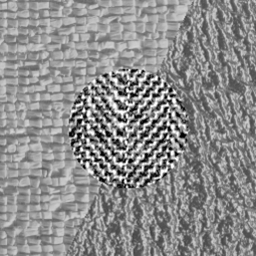
\includegraphics[width=.9\textwidth]{mosaicB.png}}
  \caption{Test Image}
\end{figure}
\end{column}
\hfill
\begin{column}{.45\textwidth}
\begin{figure}
  \colorbox{gray!20}{
\includegraphics[width=.9\textwidth]{mapB.png}}
  \caption{Ground Truth}
\end{figure}
\end{column}
\end{columns}
\end{frame}

\begin{frame}
\frametitle{K-means Initializations for B}
\begin{columns}[onlytextwidth]
\begin{column}{.45\textwidth}
\begin{figure}
  \includegraphics[width=.9\textwidth]{figs/kmeansB/kmeansgood_0_prog_B.png}
  \caption{Good}
\end{figure}
\end{column}
\hfill
\begin{column}{.45\textwidth}
\begin{figure}
  \includegraphics[width=.9\textwidth]{figs/kmeansB/kmeansbad_0_prog_B.png}
  \caption{Bad}
\end{figure}
\end{column}
\end{columns}\vfill

\begin{figure}
  \includegraphics[width=.35\textheight]{figs/kmeansB/kmeansrandom_0_prog_B.png}
  \caption{Random}
\end{figure}
\end{frame}


\begin{frame}
\frametitle{K-means Output for B}
\begin{columns}[onlytextwidth]
\begin{column}{.45\textwidth}
\begin{figure}
  \includegraphics[width=.9\textwidth]{figs/kmeansB/kmeansgood_8_prog_B.png}
  \caption{Good}
\end{figure}
\end{column}
\hfill
\begin{column}{.45\textwidth}
\begin{figure}
  \includegraphics[width=.9\textwidth]{figs/kmeansB/kmeansbad_14_prog_B.png}
  \caption{Bad}
\end{figure}
\end{column}
\end{columns}\vfill

\begin{figure}
  \includegraphics[width=.35\textheight]{figs/kmeansB/kmeansrandom_7_prog_B.png}
  \caption{Random}
\end{figure}
\end{frame}

\begin{frame}
\frametitle{K-means Performance for B}
\begin{columns}
\begin{column}{.3\textwidth}
\begin{figure}
  \includegraphics[width=.9\textwidth]{figs/kmeansB/perf_kmeansB_good.png}
  \caption{Good}
\end{figure}
\end{column}
\begin{column}{.3\textwidth}
\begin{figure}
  \includegraphics[width=.9\textwidth]{figs/kmeansB/perf_kmeansB_bad.png}
  \caption{Bad}
\end{figure}
\end{column}

\begin{column}{.3\textwidth}
\begin{figure}
  \includegraphics[width=.9\textwidth]{figs/kmeansB/perf_kmeansB_random.png}
  \caption{Random}
\end{figure}
\end{column}

\end{columns}
\end{frame}

% ------------------------------------------------------------------------------------------------------------------
\subsection{EM}
\begin{frame}
\textbf{N.B. EM initialized using the optimized output of the K-means. In this context, bad initialization for EM means the K-means was
started with bad initialization and EM initialized with the output of that K-means}
\end{frame}

\begin{frame}
\frametitle{EM Initializations by K-means for A}
\begin{columns}[onlytextwidth]
\begin{column}{.45\textwidth}
\begin{figure}
  \includegraphics[width=.9\textwidth]{figs/emA/emgood_0_prog_A.png}
  \caption{Good}
\end{figure}
\end{column}
\hfill
\begin{column}{.45\textwidth}
\begin{figure}
  \includegraphics[width=.9\textwidth]{figs/emA/embad_0_prog_A.png}
  \caption{Bad}
\end{figure}
\end{column}
\end{columns}\vfill

\begin{figure}
  \includegraphics[width=.35\textheight]{figs/emA/emrandom_0_prog_A.png}
  \caption{Random}
\end{figure}
\end{frame}


\begin{frame}
\frametitle{EM Output for A}
\begin{columns}[onlytextwidth]
\begin{column}{.45\textwidth}
\begin{figure}
  \includegraphics[width=.9\textwidth]{figs/emA/emgood_20_prog_A.png}
  \caption{Good}
\end{figure}
\end{column}
\hfill
\begin{column}{.45\textwidth}
\begin{figure}
  \includegraphics[width=.9\textwidth]{figs/emA/embad_20_prog_A.png}
  \caption{Bad}
\end{figure}
\end{column}
\end{columns}\vfill

\begin{figure}
  \includegraphics[width=.35\textheight]{figs/emA/emrandom_20_prog_A.png}
  \caption{Random}
\end{figure}
\end{frame}

\begin{frame}

\frametitle{EM Performance for A}
\begin{columns}
\begin{column}{.3\textwidth}
\begin{figure}
  \includegraphics[width=.9\textwidth]{figs/emA/perf_emA_good.png}
  \caption{Good}
\end{figure}
\end{column}
\begin{column}{.3\textwidth}
\begin{figure}
  \includegraphics[width=.9\textwidth]{figs/emA/perf_emA_bad.png}
  \caption{Bad}
\end{figure}
\end{column}

\begin{column}{.3\textwidth}
\begin{figure}
  \includegraphics[width=.9\textwidth]{figs/emA/perf_emA_random.png}
  \caption{Random}
\end{figure}
\end{column}

\end{columns}
\end{frame}

% ------------------------------------------------------------------------------------------------------------------
\begin{frame}
\frametitle{EM Initialized by K-means for B}
\begin{columns}[onlytextwidth]
\begin{column}{.45\textwidth}
\begin{figure}
  \includegraphics[width=.9\textwidth]{figs/emB/emgood_0_prog_B.png}
  \caption{Good}
\end{figure}
\end{column}
\hfill
\begin{column}{.45\textwidth}
\begin{figure}
  \includegraphics[width=.9\textwidth]{figs/emB/embad_0_prog_B.png}
  \caption{Bad}
\end{figure}
\end{column}
\end{columns}\vfill

\begin{figure}
  \includegraphics[width=.35\textheight]{figs/emB/emrandom_0_prog_B.png}
  \caption{Random}
\end{figure}
\end{frame}


\begin{frame}
\frametitle{EM Output for B}
\begin{columns}[onlytextwidth]
\begin{column}{.45\textwidth}
\begin{figure}
  \includegraphics[width=.9\textwidth]{figs/emB/emgood_12_prog_B.png}
  \caption{Good}
\end{figure}
\end{column}
\hfill
\begin{column}{.45\textwidth}
\begin{figure}
  \includegraphics[width=.9\textwidth]{figs/emB/embad_17_prog_B.png}
  \caption{Bad}
\end{figure}
\end{column}
\end{columns}\vfill

\begin{figure}
  \includegraphics[width=.35\textheight]{figs/emB/emrandom_12_prog_B.png}
  \caption{Random}
\end{figure}
\end{frame}

\begin{frame}
\frametitle{EM Performance for B}
\begin{columns}
\begin{column}{.3\textwidth}
\begin{figure}
  \includegraphics[width=.9\textwidth]{figs/emB/perf_emB_good.png}
  \caption{Good}
\end{figure}
\end{column}
\begin{column}{.3\textwidth}
\begin{figure}
  \includegraphics[width=.9\textwidth]{figs/emB/perf_emB_bad.png}
  \caption{Bad}
\end{figure}
\end{column}

\begin{column}{.3\textwidth}
\begin{figure}
  \includegraphics[width=.9\textwidth]{figs/emB/perf_emB_random.png}
  \caption{Random}
\end{figure}
\end{column}

\end{columns}
\end{frame}
% ------------------------------------------------------------------------------------------------------------------

\begin{frame}
\frametitle{K-means Vs EM on A}
\begin{columns}
\begin{column}{.3\textwidth}
\begin{figure}
  \includegraphics[width=.9\textwidth]{figs/kmeansA/perf_kmeansA_good.png}
  \caption{K-means Good}
\end{figure}
\end{column}
\begin{column}{.3\textwidth}
\begin{figure}
  \includegraphics[width=.9\textwidth]{figs/emA/perf_emA_good.png}
  \caption{EM Good}
\end{figure}
\end{column}
\end{columns}
\end{frame}

\begin{frame}
\frametitle{K-means Vs EM on B}
\begin{columns}
\begin{column}{.3\textwidth}
\begin{figure}
  \includegraphics[width=.9\textwidth]{figs/kmeansB/perf_kmeansB_good.png}
  \caption{K-means Good}
\end{figure}
\end{column}
\begin{column}{.3\textwidth}
\begin{figure}
  \includegraphics[width=.9\textwidth]{figs/emB/perf_emB_good.png}
  \caption{EM Good}
\end{figure}
\end{column}
\end{columns}
\end{frame}


\begin{frame}
\frametitle{K-means Vs EM on A}
\begin{columns}
\begin{column}{.3\textwidth}
\begin{figure}
  \includegraphics[width=.9\textwidth]{figs/kmeansA/perf_kmeansA_random.png}
  \caption{K-means Random}
\end{figure}
\end{column}
\begin{column}{.3\textwidth}
\begin{figure}
  \includegraphics[width=.9\textwidth]{figs/emA/perf_emA_random.png}
  \caption{EM random}
\end{figure}
\end{column}
\end{columns}
\end{frame}

\begin{frame}
\frametitle{K-means Vs EM on B}
\begin{columns}
\begin{column}{.3\textwidth}
\begin{figure}
  \includegraphics[width=.9\textwidth]{figs/kmeansB/perf_kmeansB_random.png}
  \caption{K-means Random}
\end{figure}
\end{column}
\begin{column}{.3\textwidth}
\begin{figure}
  \includegraphics[width=.9\textwidth]{figs/emB/perf_emB_random.png}
  \caption{EM Random}
\end{figure}
\end{column}
\end{columns}
\end{frame}

\section{Analysis}
\begin{frame}
\frametitle{Analysis}
\begin{itemize}
  \item Experiments reaffirms the fact that both K-means and EM are sensitive to initialization; good initializations have better accuracy 
  \item EM is more robust than K-means because in all cases it performs almost as good as K-means or much better than it.
  \item For example in random case K-means suffer 70\% accuracy whereas EM has 90\% accuracy
  \item The robustness is more visible in more complex segmentation for example in more complex real world image
  \item However K-means converges faster than EM
\end{itemize}
\end{frame}

\section{Real World}
\begin{frame}
\frametitle{K-means on Real Image K=6}
\includegraphics[width=.45\textwidth]{mosaicC.jpg}
\includegraphics[scale=.42]{figs/kmeansC/kmeansgood_prog_C.png}
\end{frame}

\begin{frame}
\frametitle{EM on Real Image}
\includegraphics[width=.45\textwidth]{mosaicC.jpg}
\includegraphics[scale=.42]{figs/emC/emgood_prog_C.png}
\end{frame}

\begin{frame}
\frametitle{K-means on Real Image K=4}
\includegraphics[width=.45\textwidth]{mosaicD.jpg}
\includegraphics[scale=.42]{figs/kmeansD/kmeansgood_prog_D.png}
Satellite view of Boomer Lake. K means is confused by Google's watermark. It also did not segmented the bank.
\end{frame}

\begin{frame}
\frametitle{EM on Real Image}
\includegraphics[width=.45\textwidth]{mosaicD.jpg}
\includegraphics[scale=.42]{figs/emD/emgood_prog_D.png}
EM segmented the watermark in a different cluster. Also segmented the lake, land, bank and trees.
\end{frame}

% ------------------------------------------------------------------------------------------------------------------

\end{document}

